% :Author: Stefan Kottwitz
% :Source: TeXblog - TikZ: shaded cube
%          http://texblog.net/latex-archive/graphics/tikz-cube-3d/
\documentclass[12pt]{standalone}
\usepackage{tikz}
\usepackage{tikz-3dplot}
\usepackage{verbatim}

\begin{comment}

:Title: Sudoku 3D cube
:Tags: 3D, Transformations

This example shows how to create an effective 3D effect using the ``slant`` transformation.
Shading has been added to enhance the 3D impression. Read more about this example over
at TeXblog_.

.. _TeXblog: http://texblog.net/latex-archive/graphics/tikz-cube-3d/

:Author: Stefan Kottwitz
:Source: `TeXblog - TikZ: shaded cube`__

.. __: http://texblog.net/latex-archive/graphics/tikz-cube-3d/

\end{comment}

\usetikzlibrary{positioning}
\begin{document}
\large
\pagestyle{empty}
\definecolor{pfb}{RGB}{38, 115, 184}
\definecolor{ucsdblue}{HTML}{182b49}
%171, 142, 5
\definecolor{ucsdgold}{HTML}{C69214}
%rgb(24,43,73)
\resizebox {5in} {!} {
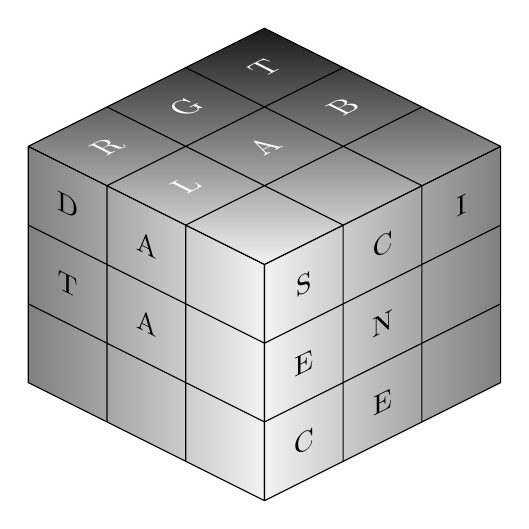
\begin{tikzpicture}[every node/.style={minimum size=1cm},on grid]
\begin{scope}[every node/.append style={yslant=-0.5},yslant=-0.5]
  \shade[right color=black!5, left color=black!50] (0,0) rectangle +(3,3);
  \node[text=black ] at (0.5,2.5) {D};
  \node[text=black ] at (1.5,2.5) {A};
  \node[text=black ] at (2.5,2.5) {};
  \node[text=black ] at (0.5,1.5) {T};
  \node[text=black ] at (1.5,1.5) {A};
  \node[text=black ] at (2.5,1.5) {};
  \node[text=black ] at (0.5,0.5) {};
  \node[text=black ] at (1.5,0.5) {};
  \node[text=black ] at (2.5,0.5) {};
  \draw (0,0) grid (3,3);
\end{scope}
\begin{scope}[every node/.append style={yslant=0.5},yslant=0.5]
  \shade[right color=black!50,left color=black!5] (3,-3) rectangle +(3,3);
  \node[text=black ] at (3.5,-0.5){S};
  \node[text=black ] at (4.5,-0.5) {C};
  \node[text=black ] at (5.5,-0.5) {I};
  \node[text=black ] at (3.5,-1.5) {E};
  \node[text=black ] at (4.5,-1.5){N};
  \node[text=black ] at (5.5,-1.5) {};
  \node[text=black ] at (3.5,-2.5) {C};
  \node[text=black ] at (4.5,-2.5) {E};
  \node[text=black ] at (5.5,-2.5) {};
  \draw(3,-3) grid (6,0);
\end{scope}
\begin{scope}[every node/.append style={
    yslant=0.5,xslant=-1},yslant=0.5,xslant=-1
  ]
  \shade[bottom color=black!5, top color=black!90] (6,3) rectangle +(-3,-3);
  \node[text=white] at (3.5,2.5) {R};
  \node[text=white] at (3.5,1.5) {L};
  \node[text=white] at (3.5,0.5) {};
  \node[text=white] at (4.5,2.5) {G};
  \node[text=white] at (4.5,1.5) {A};
  \node[text=gray]at (4.5,0.5) {};
  \node[text=white] at (5.5,2.5) {T};
  \node[text=white] at (5.5,1.5) {B};
  \node[text=gray]at (5.5,0.5) {};
  \draw[text=black] (3,0) grid (6,3);
\end{scope}
\end{tikzpicture}
}


%\tdplotsetmaincoords{60}{125}
%\begin{tikzpicture}[
%		tdplot_main_coords,
%		grid/.style={very thin,gray},
%		axis/.style={->,blue,thick},
%		cube/.style={very thick,fill=red},
%		cube hidden/.style={very thick,dashed}]
%	%draw a grid in the x-y plane
%	\foreach \x in {-0.5,0,...,2.5}
%		\foreach \y in {-0.5,0,...,2.5}
%		{
%			\draw[grid] (\x,-0.5) -- (\x,2.5);
%			\draw[grid] (-0.5,\y) -- (2.5,\y);
%		}

%	%draw the axes
%	\draw[axis] (0,0,0) -- (3,0,0) node[anchor=west]{$x$};
%	\draw[axis] (0,0,0) -- (0,3,0) node[anchor=west]{$y$};
%	\draw[axis] (0,0,0) -- (0,0,3) node[anchor=west]{$z$};

%	%draw the front-right of the cube
%	\draw[cube] (2,0,0) -- (2,2,0) -- (2,2,2) -- (2,0,2) -- cycle;

%	%draw the front-left of the cube
%	\draw[cube] (0,2,0) -- (2,2,0) -- (2,2,2) -- (0,2,2) -- cycle;

%	%draw the top of the cube
%	\draw[cube] (0,0,2) -- (0,2,2) -- (2,2,2) -- (2,0,2) -- cycle;

%	%draw dashed lines to represent hidden edges
%	\draw[cube hidden] (0,0,0) -- (2,0,0);
%	\draw[cube hidden] (0,0,0) -- (0,2,0);
%	\draw[cube hidden] (0,0,0) -- (0,0,2);

%\end{tikzpicture}

\end{document}
